\chapter{Method of Approach}
\label{ch:method}

This chapter describes the implementation of AFLuent and the experiment setup and
execution process. More specifically, the reasoning behind design decisions and
the result are the main focus. Additionally, charts and diagrams  are used to
demonstrate the the algorithms, structure, and flow of execution.

\section{Development Environment and Toolset}
\label{sec:DevEnviron}

Prior to explain how implementation was completed, a ground-up overview of the
tools used and their roles is necessary to establish definitions and facilitate
the understanding of how dependencies they are connected. AFLuent being a Python
tool allows its development to rely on a wide variety of helpful and popular
tools. Some of the most important tools and dependencies are discussed below.

\subsection{Poetry}
\label{subsec:poetry}

Poetry is a Python virtual environment management tool that allows developers to
set up an isolated environment for their projects. Furthermore, it manges the
installation of Python dependencies on the virtualenv and updates them when
necessary. Poetry has a crucial role in the implementation of AFLuent since it's
used to make the development process simpler, its role also goes beyond
that to the packaging and publishing of AFLuent to the Python Package Index
(PyPI). Poetry's ability to abstract and simplify all the details in creating a
Python package, makes it essential for development. However, from a user's
perspective, Poetry is not necessary to run or use the tool for fault localization.

\subsection{Pytest}
\label{subsec:pytest}

Pytest is a Python testing framework used to write and execute a variety of
tests, especially unit tests. Many developers in the community have contributed
to Pytest through plugins that extend Pytest's functionality and allow it to
accomplish new beneficial tasks. As mentioned previously, AFLuent is a Pytest
plugin that adds automated fault localization features. By definition, AFLuent
relies on Pytest in order to function properly. More details on how AFLuet is
integrated with pytest can be found in Section \ref{sec:makingPytestPlugin}.

\subsection{Coverage.py}
\label{subsec:coverage}

Spectrum-based fault localization requires data on code coverage and test
results in order to calculate and rank suspicious of elements in the code.
Coverage.py\cite{coverage_py_website} is a Python tool that provides an easy to use application
programming interface to collect that data. The tool also provides various
configuration for the user to skip certain file or directories from being
considered. AFLuent relies on this tool to calculate what's known as per-test
coverage. This data describes the lines of code covered by a single test case
and organized in an accessible way to find out the number of passing and failing
test cases that executed each line. Automated fault localization approaches
require this information in order to calculate suspiciousness scores and
Coverage.py can provide that relatively easily.

\subsection{Radon}
\label{subsec:radon}

Radon is a Python tool used to calculate metrics of code complexity.
Specifically, it's used in AFLuent to calculate cyclomatic complexity of some
elements to break ties in rankings. When the user requests that AFLuent
considers cyclomatic complexity to be considered when breaking ties, Radon is
used to create a dataset of complexity scores. Since single lines cannot have a
cyclomatic complexity score, they are assigned the score of the function they're
a part of. Furthermore, the dataset is organized to facilitate efficient
searching by the line number in question.

\subsection{Libcst}
\label{subsec:libcst}

In order to provide additional methods to breaking ties between element
rankings, Libcst is used to create an abstract syntax tree of the code in
question. This approach allows AFLuent to detect error prone syntax and
formulate a score to use to break ties between lines if the need arises.
Additional details on the use of Libcst are discussed in section
\ref{sec:tiebreaking}: Tie Breaking.

\section{AFLuent as a Pytest Plugin}
\label{sec:makingPytestPlugin}

\begin{figure}[!htb]
	\begin{center}
		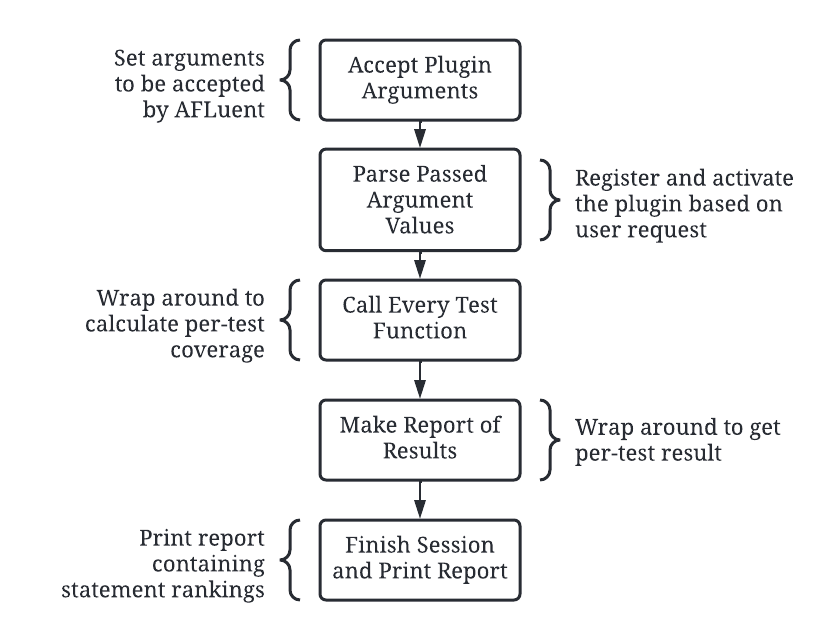
\includegraphics[width=11.9cm]{pytest_flowfchart.png}
		\caption{\label{fig:pytest_flow} Pytest Tasks Flowchart}
	\end{center}
\end{figure}

Pytest provides simple and intuitive ways of extending its functionality through
hooks. These hooks break up the standard Pytest execution steps and allow
external code to run at these points. A plugin is essentially a collection of
packaged hooks that fit in the workflow of Pytest. AFLuent makes use of five
different hooks to implement automated fault localization.
Figure \ref{fig:pytest_flow} shows a general overview of the steps changed in the
workflow of Pytest. Additionally, the section below describes in details how each
step was modified.

\section{Installing AFLuent}
\label{subsec:afluent_install}

As part of the goal of creating a novice friendly tool, it's very important that
AFLuent can be installed and set up easily on any system with little to no
complications. To achieve that, AFLuent is published to the Python Package Index
(PyPI), which makes it installable through the \code{pip install afluent}
command. Once this command runs successfully, AFLuent is automatically
integrated with Pytest as a plugin and will be ran with every pytest session
unless otherwise disabled intentionally. AFLuent's dependency on Coverage.py
creates a small but avoidable conflict. In the case that AFluent and another plugin that
utilizes Coverage.py is active in the same Pytest session, various errors might
occur where coverage information is not calculated correctly, thus affecting the
automated fault localization process. This issue was prevalent when specifically
using \code{pytest-cov} plugin, which produces a coverage report at the end of a
Pytest session. AFLuent handles this problem by checking for the presence of
other Coverage.py reliant plugins and warns the user. Due to this issue,
AFLuent will not run in the session unless specified specifically using the
command-line arguments discussed in the following section.

\subsection{Adding Command-Line Arguments}
\label{subsec:pytest_cli}

Pytest already supports a multitude of command line arguments that allow the
user to pass configuration that change how the test suite is executed and
reported. Similarly, AFLuent requires user passed arguments to complete a
variety of tasks. The hook \code{pytest\_addoption} allows adding new
arguments in a fashion similar to the \code{argparse} Python library.
The \code{argparse} library supports features that allow easy parsing and validation of
command-line arguments. Furthermore, it facilitates working with input with
various data types.
The added arguments accept values that specify the following:
\begin{itemize}
    \item If AFLuent should be enabled for the current Pytest session.
    \begin{itemize}
        \item Flags: \code{---afl-debug} or \code{---afl}
    \end{itemize}
    \item The techniques for suspiciousness score calculations
    \begin{itemize}
        \item \code{---tarantula}: enable fault localization using Tarantula approach
        \item \code{---ochiai}: enable fault localization using Ochiai approach
        \item \code{---ochiai2}: enable fault localization using Ochiai2 approach
        \item \code{---dstar}: enable fault localization using DStar approach
        \item \code{---dstar-pow}: used to set the power to use in the DStar
        approach. Defaults to 3
        \item Multiple approaches can be used at the same time, however, results
        will be sorted by the approach passed first.
    \end{itemize}
    \item The number of results to display in the report
    \begin{itemize}
        \item \code{---afl-results}: number of top results to show in the
        terminal window. Defaults to 20
    \end{itemize}
    \item The directories and files to be ignored while calculating coverage
    \begin{itemize}
        \item \code{---afl-ignore}: Used to pass directories and files to
        ignore. Example: \code{tests/*} will ignore all files and directories
        inside the \code{tests} folder.
    \end{itemize}
    \item The types of file reports to created after the Pytest session is over
    \begin{itemize}
        \item \code{---report}: accepts \code{json} or \code{csv} and generate
        reports with the passed format.
        \item \code{---per-test-report}: requires that a per-test coverage
        report is produced. This report is only generated in JSON format.
    \end{itemize}
    \item The tie breaking approaches to resolve ties in rankings
    \begin{itemize}
        \item \code{---tiebreaker}: allowed values are \code{random},
        \code{cyclomatic}, \code{logical},

		or \code{enhanced}
		\item Defaults to \code{random} if no approach is passed.
    \end{itemize}
\end{itemize}

\subsection{Activating AFLuent}
\label{subsec:activate_afluent}

After arguments are passed, the next steps parses through some of them to check
if AFLuent was enabled and to validate some of their values. The Pytest hook
\code{pytest\_cmdline\_main} gives access to the collected configuration. In
this hook, checks are conducted to see if there are other active plugins that
utilize Coverage.py. These checks are necessary due to conflicts in collecting
data when multiple plugins use Coverage.py simultaneously. The problem is
resolved through warnings to the user that ask to disable these plugins in order
for AFLuent to run properly. Lastly, if AFLuent is enabled, an \code{Afluent} object is initialized
with the passed configuration and registered as a plugin for the current Pytest session.

\subsection{Calculating Per-test Coverage and Test Result}
\label{subsec:calculate_coverage}

Per-test coverage is defined here as the collection of lines executed by
each individual test case. In order to collect this data, AFLuent adds a wrapper
that executes code before and after each test case function is called. The
\code{pytest\_pyfunc\_call} hook is used in this scenario. The execution steps
are as follows:

\begin{enumerate}
    \item \code{cov.start()} begins recording coverage
    \item the hook yields back control to Pytest which calls the individual test case
    \item \code{cov.stop()} stops recording coverage
    \item The collected data is then organized in a simpler structure defined as
    the program spectra
    \item The process repeats for every test case
\end{enumerate}

Once per-test coverage is completed, the \code{pytest\_runtest\_makereport} hook
is used to get the outcome of each test case and add it to the program spectra
structure. There are three possible test outcome in Pytest, `Passed', `Failed',
and `Skipped'.

\subsection{Reporting Results}
\label{subsec:report_results}

The last step in AFLuent execution as part of Pytest is to report the fault
localization outcome. The \code{pytest\_sessionfinish} hook is used to detect the
exit code of the session and display output on the console accordingly. An exist
code of 0 means that all tests have passed and there is no need to perform fault
localization, therefore, a message would display that to the user before
finishing the Pytest run. On the other hand an exit code of 1, would indicate
that at least one test case failed during the pytest session. In this scenario,
AFLuent initializes a \code{Spectrum} object, which is responsible for parsing
through the program spectra structure, ranking elements based on suspiciousness,
and producing an output to the console.

\section{AFLuent's Components}
\label{sec:components}

Considering all the steps involved in calculating and reporting suspiciousness
of elements, AFLuent is implemented in an object oriented style that focuses on
the readability and maintainability of the code. By splitting up AFLuent to a
collection of objects organized in a hierarchy, the testing approach becomes more
clear and debugging becomes easier. This section discusses the objects oriented
structure starting with the least complex.

\subsection{Line Object}
\label{subsec:line_obj}

A line is the simplest unit in a large project or program. With that in mind, a
\code{Line} object describes the attributes and implements the functionalities
associated with a single line in the context of automated fault localization.
Important attributes of a line include identifiers such as the line number and
file path it belongs to. Other line-specific information include a list of
failed test cases that executed this line, and another for tests that passed.
This information is crucial in calculating suspiciousness scores. These scores are also stored as
attributes of each Line object. Another stored attribute is a collection of
scores used to break ties between lines when their suspiciousness is the same.
In general, these scores measure how error prone is the code with the current
syntax structure. Further discussion on breaking ties using these scores can be
found in Section \ref{sec:tiebreaking} Tie breaking.

As for functions, a Line object contains an implementation of the four
equations, Tarantula shown in Figure \ref{fig:tarantulaEquation}, Ochiai shown in
Figure \ref{fig:ochiaiEquation}, Ochiai2 shown in Figure \ref{fig:ochiai2Equation},
and DStar shown in Figure \ref{fig:dstarEquation},
where suspiciousness scores are calculated and rounded up to four decimal places.
The mathematical implementations of these functions also handle and account for
division by zero. Depending on the equation, there could be multiple instances
where division by zero is possible. The following subsections discuss how this
issue was handled for each equation.

\subsubsection{Division by Zero: Tarantula}
\label{subsubsec:div_by_zero_taran}
In the Tarantula equation, division by zero occurs if either the number of
total passing tests or number of total failing tests is zero. In the case that
there are no failing test-cases in the whole test suite, then the suspiciousness
of all covered statements is zero (not suspicious) since there was no fault. The
other edge case occurs when there are no passing tests in the whole test suite,
in which every covered line has the maximum suspiciousness of 1. It is important
to acknowledge that the outcomes reached here only apply to code that has been
covered by the test suite. Faulty lines, which are not covered by any test case
will not be investigated since there is no data to calculate their
suspiciousness. Using values plugged in to Figure \ref{fig:tarantulaEquation}, the
examples in Figure \ref{fig:taran_div_by_zero_1} and Figure \ref{fig:taran_div_by_zero_2} show
the two possible cases where division by zero might occur in the Tarantula
equation.

\begin{figure}[!htb]
	\begin{center}
        When \textbf{N$_{CF}$ = 0} and \textbf{N$_{UF}$ = 0 }
		\begin{equation}
			Tarantula(element) = \frac{\frac{\textbf{0}}{\textbf{0}}}{\frac{\textbf{N$_{CS}$}}{\textbf{N$_{CS}$}+\textbf{N$_{US}$}} + \frac{\textbf{0}}{\textbf{0}}}
		\end{equation}
		\caption{\label{fig:taran_div_by_zero_1} Tarantula Division by Zero Example 1}
	\end{center}
\end{figure}

\begin{figure}[!htb]
	\begin{center}
        When \textbf{N$_{CS}$ = 0} and \textbf{N$_{US}$ = 0 }
		\begin{equation}
			Tarantula(element) = \frac{\frac{\textbf{N$_{CF}$}}{\textbf{N$_{CF}$} + \textbf{N$_{UF}$}}}{\frac{\textbf{0}}{\textbf{0}} + \frac{\textbf{N$_{CF}$}}{\textbf{N$_{CF}$}+\textbf{N$_{UF}$}}}
		\end{equation}
		\caption{\label{fig:taran_div_by_zero_2} Tarantula Division by Zero Example 2}
	\end{center}
\end{figure}

Figure \ref{fig:taran_div_by_zero_1} shows the case where there is a total of zero
failed test cases, covering AND not covering the element, in which a score
of 0 is assigned to the element. On the other hand,
Figure \ref{fig:taran_div_by_zero_2} shows the case where there is a total of zero
passing test cases, in which a maximum score of 1 is assigned to the element.

\subsubsection{Division by Zero: Ochiai}
\label{subsubsec:div_by_zero_ochiai}

Division by zero occurs in the Ochiai formula when there is not test coverage
information for a line or when the total number of failed tests is zero.
The latter case indicates that the line is not suspicious since it did not
cause any failures, therefore, zero is returned as the suspiciousness score.
However, the former case is not considered at all since AFLuent does not include
lines with no coverage information.
Figure \ref{fig:ochiai_div_by_zero_1} and Figure \ref{fig:ochiai_div_by_zero_2}
demonstrates that equation after plugging in
the zero values from \ref{fig:ochiaiEquation}

\begin{figure}[!htb]
	\begin{center}
        When \textbf{N$_{CF}$ = 0} and \textbf{N$_{UF}$ = 0 }
		\begin{equation}
			Ochiai(element) = \frac{\textbf{0}}{\sqrt{(\textbf{0}) \cdot (\textbf{0}  + \textbf{N$_{CS}$})}}
		\end{equation}
		\caption{\label{fig:ochiai_div_by_zero_1} Ochiai Division by Zero Example 1}
	\end{center}
\end{figure}

\begin{figure}[!htb]
	\begin{center}
        When \textbf{N$_{CF}$ = 0} and \textbf{N$_{CS}$ = 0 }
		\begin{equation}
			Ochiai(element) = \frac{\textbf{0}}{\sqrt{(\textbf{0}  + \textbf{N$_{UF}$}) \cdot (\textbf{0})}}
		\end{equation}
		\caption{\label{fig:ochiai_div_by_zero_2} Ochiai Division by Zero Example 2}
	\end{center}
\end{figure}

Figure \ref{fig:ochiai_div_by_zero_1} is an example of when there is zero total
failed test cases, resulting in a zero suspiciousness score.
However Fig\ref{fig:ochiai_div_by_zero_2} shows an example where there is no
failed or successful tests that cover the line. This scenario does not
occur in AFLuent, which only looks at lines that have some coverage data through
passing or failing tests. Therefore, it wasn't necessary to handle this possibility.

\subsubsection{Division by Zero: Ochiai2}
\label{subsubsec:div_by_zero_ochiai2}

Considering the number of terms in the denominator of the formula to calculate
score using Ochiai2, there are technically four instances where the denominator
can be zero. In the first case, no tests, failing or passing, cover the
statement. More formally when \textbf{N$_{CF}$ + N$_{CS}$ = 0}.
Figure \ref{fig:ochiai2_div_by_zero_1} shows the equation with the zero plugged in.
While this is an issue mathematically, it does not occur in AFLuent because the
tool only analyzes elements that have been covered at least once by a failing or
a passing test. Therefore, there is no need to handle this possibility.

\begin{figure}[!htb]
	\begin{center}
		\begin{equation}
			Ochiai2(element) = \frac{\textbf{N$_{CF}$}\cdot{\textbf{N$_{US}$}}}{\sqrt{(\textbf{0}) \cdot (\textbf{N$_{US}$}  + \textbf{N$_{UF}$}) \cdot (\textbf{N$_{CF}$}  + \textbf{N$_{UF}$}) \cdot (\textbf{N$_{CS}$}  + \textbf{N$_{US}$})}}
		\end{equation}
		\caption{\label{fig:ochiai2_div_by_zero_1} Ochiai2 Division by Zero
		Example 1}
	\end{center}
\end{figure}

Moving on to the next possibility of division by zero, which occurs when
\textbf{N$_{US}$ + N$_{UF}$ = 0}. In this case, there are no tests that do not
cover the element being inspected, or in other words, all the tests (both
failing and passing) do cover this element. Considering that \textbf{N$_{US}$}
is a zero in this case, it would cause the numerator to be a zero and result in
a zero divided by zero. Due to both numerator and denominator being zero, the
suspiciousness score output is also returned as zero.

\begin{figure}[!htb]
	\begin{center}
		\begin{equation}
			Ochiai2(element) = \frac{\textbf{N$_{CF}$}\cdot{\textbf{N$_{US}$}}}{\sqrt{(\textbf{N$_{CF}$}  + \textbf{N$_{CS}$}) \cdot (\textbf{0}) \cdot (\textbf{N$_{CF}$}  + \textbf{N$_{UF}$}) \cdot (\textbf{N$_{CS}$}  + \textbf{N$_{US}$})}}
		\end{equation}
		\caption{\label{fig:ochiai2_div_by_zero_2}  Ochiai2 Division by Zero
		Example 2}
	\end{center}
\end{figure}

In the third possibility where a division by zero could happen, the third term
\textbf{N$_{CF}$ + N$_{UF}$ = 0}. This would mean that there are a total of zero
failed tests that both cover and not cover the element. Since AFLuent will only
run when there is at least one failure, this situation is not possible during
the tool's runtime. Figure  \ref{fig:ochiai2_div_by_zero_3} shows the zero as part
of the full equation.

\begin{figure}[!htb]
	\begin{center}
		\begin{equation}
			Ochiai2(element) = \frac{\textbf{N$_{CF}$}\cdot{\textbf{N$_{US}$}}}{\sqrt{(\textbf{N$_{CF}$}  + \textbf{N$_{CS}$}) \cdot (\textbf{N$_{US}$}  + \textbf{N$_{UF}$}) \cdot (\textbf{0}) \cdot (\textbf{N$_{CS}$}  + \textbf{N$_{US}$})}}
		\end{equation}
		\caption{\label{fig:ochiai2_div_by_zero_3} Ochiai2 Division by Zero
		Example 3}
	\end{center}
\end{figure}

The last possibility where division by zero in Ochiai2 can occur is when
\textbf{N$_{CS}$ + N$_{US}$ = 0}, in which there are zero total successful test
cases. In this situation, there is no indicator of correct functionality and
therefore every element is highly suspicious. A score of 1.0 will always be
returned in this scenario. Figure  \ref{fig:ochiai2_div_by_zero_4} shows the
equation with the zero in the denominator.

\begin{figure}[!htb]
	\begin{center}
		\begin{equation}
			Ochiai2(element) = \frac{\textbf{N$_{CF}$}\cdot{\textbf{N$_{US}$}}}{\sqrt{(\textbf{N$_{CF}$}  + \textbf{N$_{CS}$}) \cdot (\textbf{N$_{US}$}  + \textbf{N$_{UF}$}) \cdot (\textbf{N$_{CF}$}  + \textbf{N$_{UF}$}) \cdot (\textbf{0})}}
		\end{equation}
		\caption{\label{fig:ochiai2_div_by_zero_4} Ochiai2 Division by Zero
		Example 4}
	\end{center}
\end{figure}

\subsubsection{Division by Zero: DStar}
\label{subsubsec:div_by_zero_dstar}

In the DStar equation, division by zero takes place only in one case. When the
number of passing test cases that cover the line AND the number of failed test
cases that do not cover the line are both zero, the denominator evaluates to
zero. This translates to the following: if there is no passing tests executing
this line and no failing test executing other lines only, then this line should
have the maximum suspiciousness score possible. However, since DStar has a
numerator raised to a power set by the user, it has no numerical upper limit on
the resulting score. To resolve this issue, the maximum integer value is
assigned as the suspiciousness score of this line.
Figure \ref{fig:dstar_div_by_zero} shows and example of this scenario after
plugging in values from Figure \ref{fig:dstarEquation}

\begin{figure}[!htb]
	\begin{center}
        When \textbf{N$_{CS}$ = 0} and \textbf{N$_{UF}$ = 0 }
		\begin{equation}
			Dstar(element) = \frac{(\textbf{N$_{CF}$})^{\ast}}{\textbf{0}}
		\end{equation}
		\caption{\label{fig:dstar_div_by_zero} DStar Division by Zero Example}
	\end{center}
\end{figure}

\subsection{ProjFile Object}
\label{subsec:projfile_obj}

ProjFile objects are designed to contain attributes that describe whole files.
Additionally, they support functionality that apply to these files. The most
important attributes of these objects is the \code{lines} instance variable,
which stores a dictionary of contents of the file. Specifically, the keys in
this dictionary are line numbers in the file and the values are the Line objects
discussed previously. In addition to storing this data, ProjFile implements an
intuitive way to update it with a new result of a test case. \code{update\_file}
function takes in a list of numbers of covered lines executed by a test case as well as the
result and the name of that test case. Following that, it iterates through the
covered line numbers and updates the Line objects stored in the ProjFile
dictionary. This approach creates a hierarchy between the objects by nesting
Line objects inside of ProjFile objects.

\subsection{Spectrum Object}
\label{subsec:spectrum_obj}

This object contains some of the core functionalities that organizes the
collected data and displays it to the console. Similar to how a ProjFile object
stores a dictionary of line number and Line object pairs, Spectrum takes nesting
a step further and stores a dictionary of file paths and ProjFile objects as
key-value pairs. Additionally, it keeps track of running totals of passed,
failed, and skipped test cases, which are used to calculate suspiciousness
scores. Lastly, it's responsible for sorting Line objects in a descending order
from highest suspiciousness scores. Once this task is completed, the Spectrum
object produces a table formatted report with color coded results that
demonstrate to the user the outcome of fault localization.

\subsection{Afluent Object}
\label{subsec:afluent_obj}

While this Object does not implement any functionality regarding the calculation
or sorting of suspiciousness scores, it plays an important role in integrating
this tool with Pytest. By containing several of the Pytest hooks mentioned
prior, this object is registered as the plugin when AFLuent is enabled through
command line arguments. Following the end of the Pytest session, the AFluent
object initializes a Spectrum Object and forwards the arguments collected from
the console command. Following that, it calls the Spectrum object to produce and
print its report. Overall, this object acts as a pipeline that passes coverage
information and command line arguments collected from the Pytest session to the
infrastructure responsible for performing fault localization.

\subsection{Objects Overview}
\label{subsec:obj_overview}

\begin{figure}[!htb]
	\begin{center}
		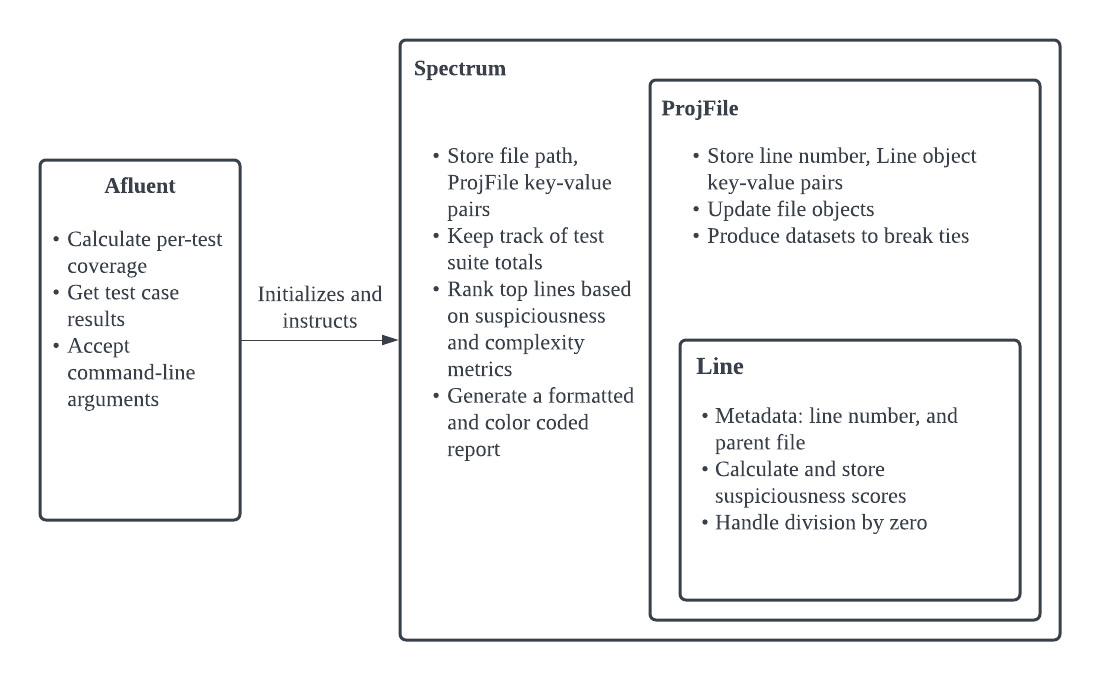
\includegraphics[width=15.5cm]{object_oriented_structure.png}
		\caption{\label{fig:oop_structure} AFLuent Object Structure}
	\end{center}
\end{figure}

Fig\ref{fig:oop_structure} provides a visual simplification of the different
components of AFluent and an overview of their roles in the functioning of the
tool. Overall the nested structure creates several layers that facilitate
development by isolating the different components and hiding unnecessary
information from other objects in the hierarchy. By following this structures,
unit tests can be written much easier and debugging becomes a simpler task.

\section{AFLuent's Output}
\label{sec:afluent_output}

While the main purpose of AFLuent is to produce a report of the most suspicious
statements, there are many additional features that can increase the readability
and user friendliness of the report. The input and workflow of AFLuent was
discussed in the previous sections, this section focuses on the outcome and
discusses how the user should interact with it.

\subsection{Feedback Messages}
\label{subsec:feedback_messages}

Throughout the execution of AFLuent, unexpected things can occur. And while
Python and Pytest error messages can be produced, AFLuent also shows console
output that gives a hint regarding what went wrong. There are three tiers of
messages produced by AFLuent, Error, Warning, and Success messages, each color
coded using red, orange, and green respectively. Each one is designed to stand
out to the user and provide a clear and concise description of the scenario.

\subsubsection{Success Messages}
\label{subsubsec:success_message}

This message is produced in the case that the test suite passes with no
error or failures. Using bright green highlighted message with bold white
letters, the message displays: \code{All tests passed, no need to diagnose using
AFLuent}. Fig\ref{fig:success_message} demonstrates the success message output
when AFLuent is ran on the project's test suite.

\begin{figure}[!htb]
	\begin{center}
		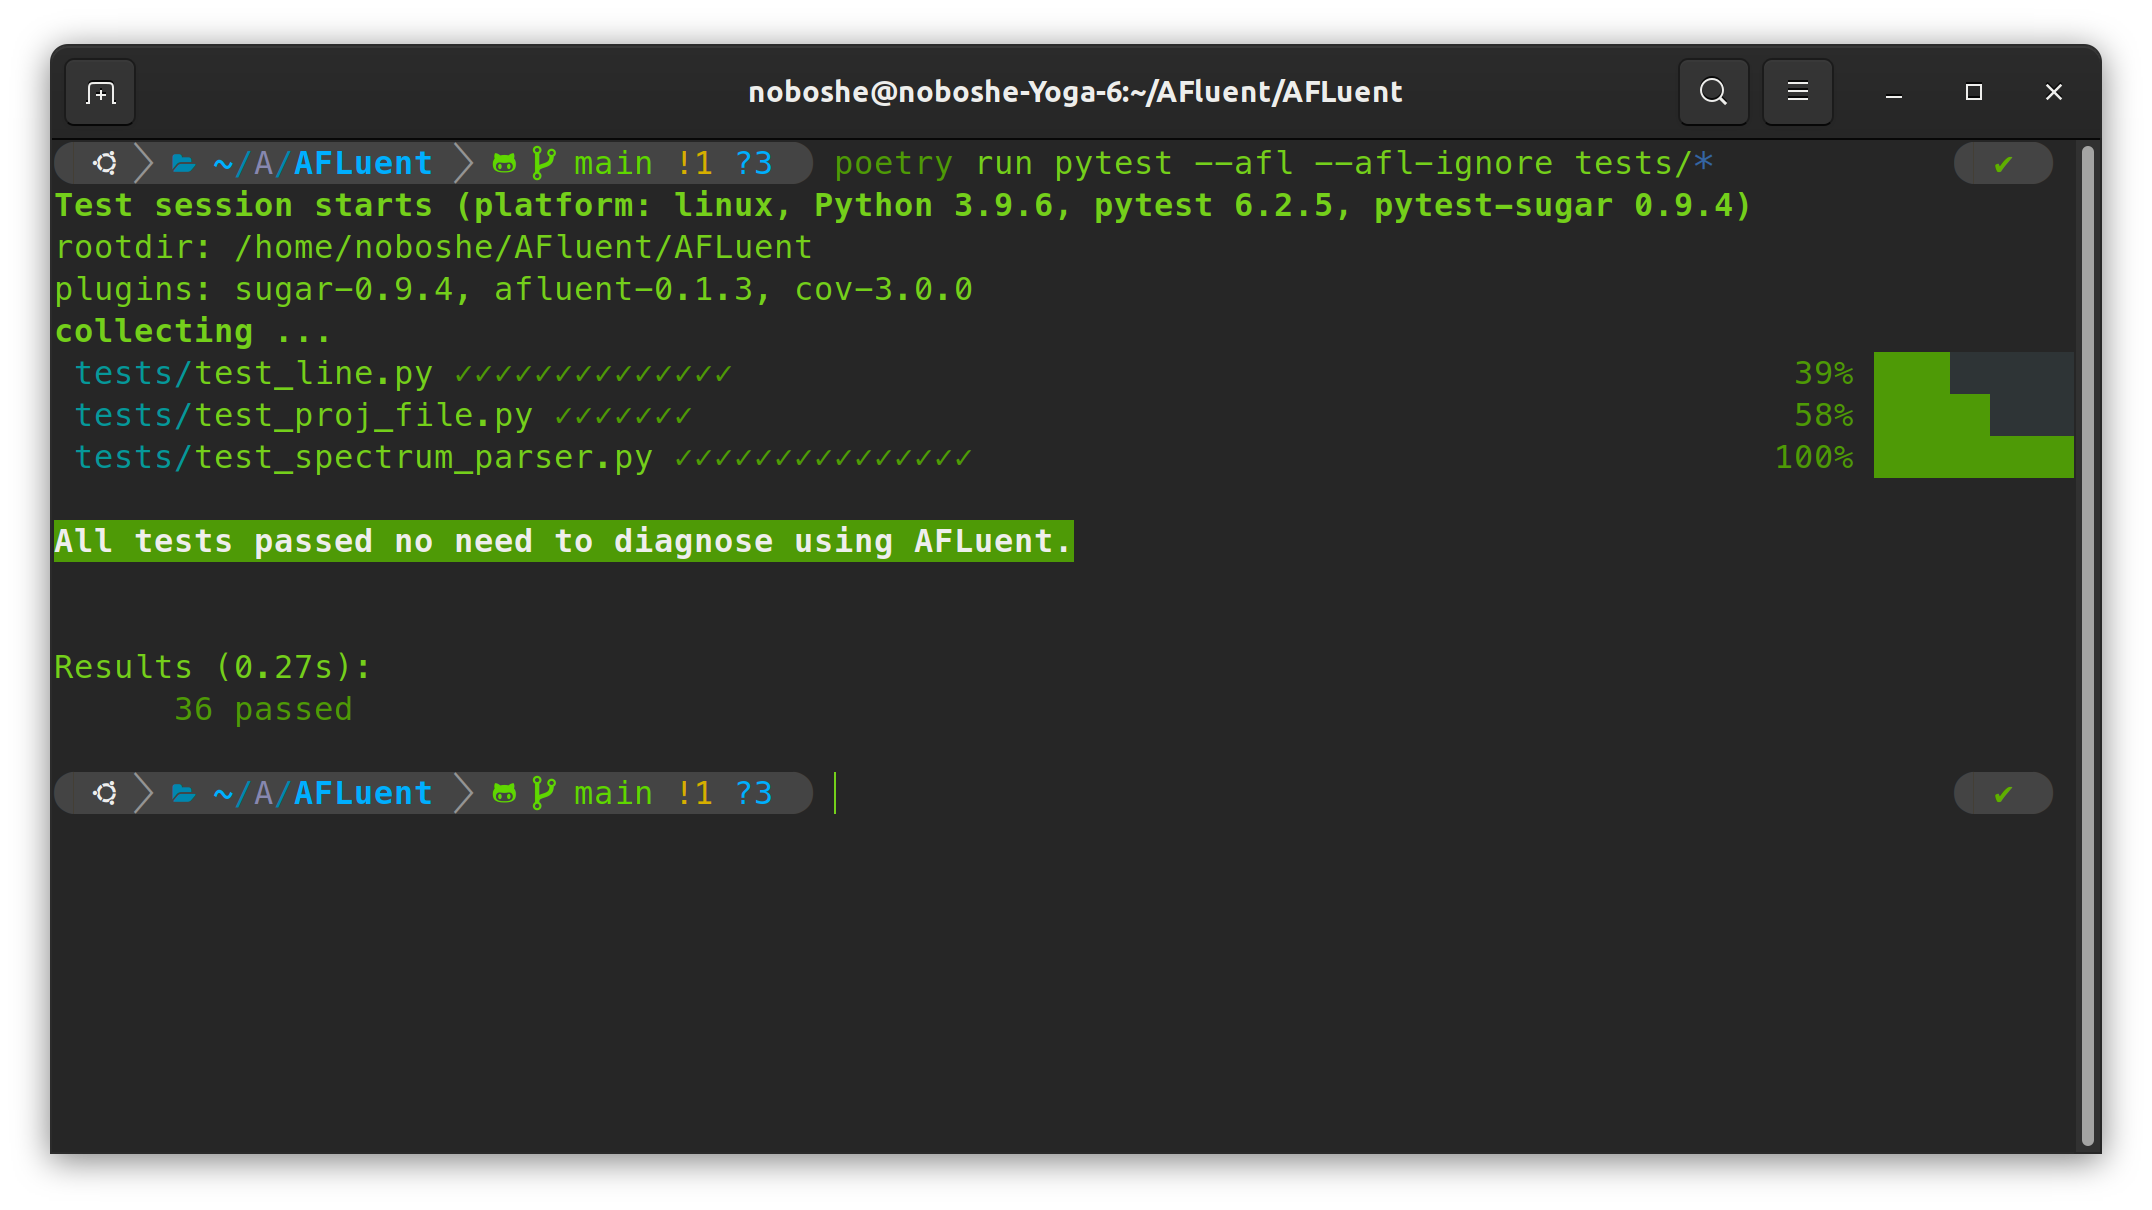
\includegraphics[width=15.5cm]{success_message.png}
		\caption{\label{fig:success_message} Example of Success Message}
	\end{center}
\end{figure}


\subsubsection{Error Messages}
\label{subsubsec:error_message}

Unlike success messages, error messages are produced when things aren't going as
expected. However, in this case, they aren't meant to denote complete failure of
AFLuent, but rather to communicate a major alert to the user. This type of
message is produced when the Pytest session exists with status code 1, which
occurs when at least one test fails. Figure \ref{fig:error_message} shows the
console output when a test failure was purposefully introduced. A bright red
highlighted message with bold white letters indicate that fault localization
using AFLuent is underway.

\begin{figure}[!htb]
	\begin{center}
		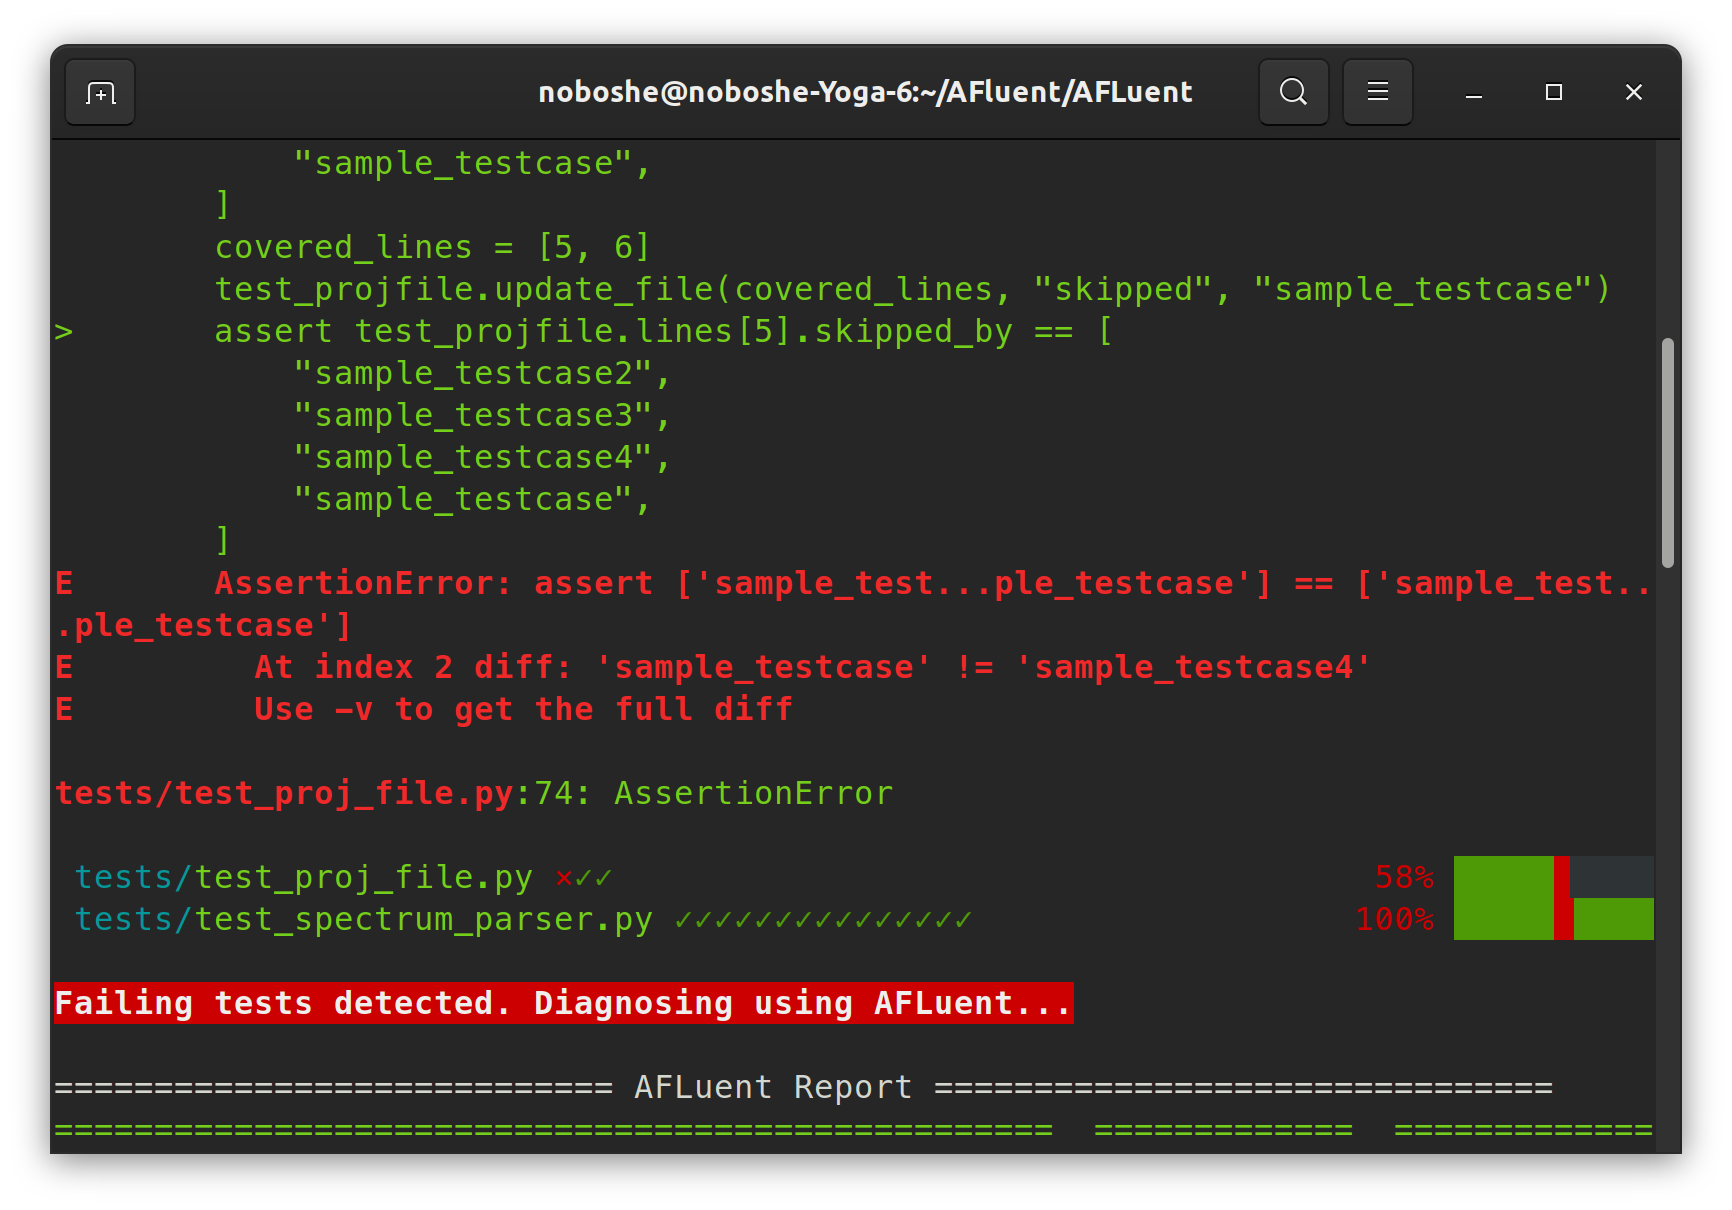
\includegraphics[width=15.5cm]{error_message.png}
		\caption{\label{fig:error_message} Example of Error Message}
	\end{center}
\end{figure}

\subsubsection{Warning Messages}
\label{subsubsec:warning_message}

The last type of messages produced during the runtime of AFLuent are warning
messages. They communicate important information to the user but do not signify
a major problem. Warning messages are displayed in three possible scenarios. In
the case that the user passes the \code{-x} or \code{---maxfail} command line
arguments to Pytest, the session can stop at the first test failure. This is
problematic from a fault localization standpoint because it prevents further
collection of coverage information and test outcomes from the rest of the test
suite. In order to let the user be aware of this issue, the warning message
shown in Figure \ref{fig:warning_message_1} is displayed. Regardless, AFLuent will
continue running with standard behavior, however, results are very likely to be
inaccurate.

\begin{figure}[!htb]
	\begin{center}
		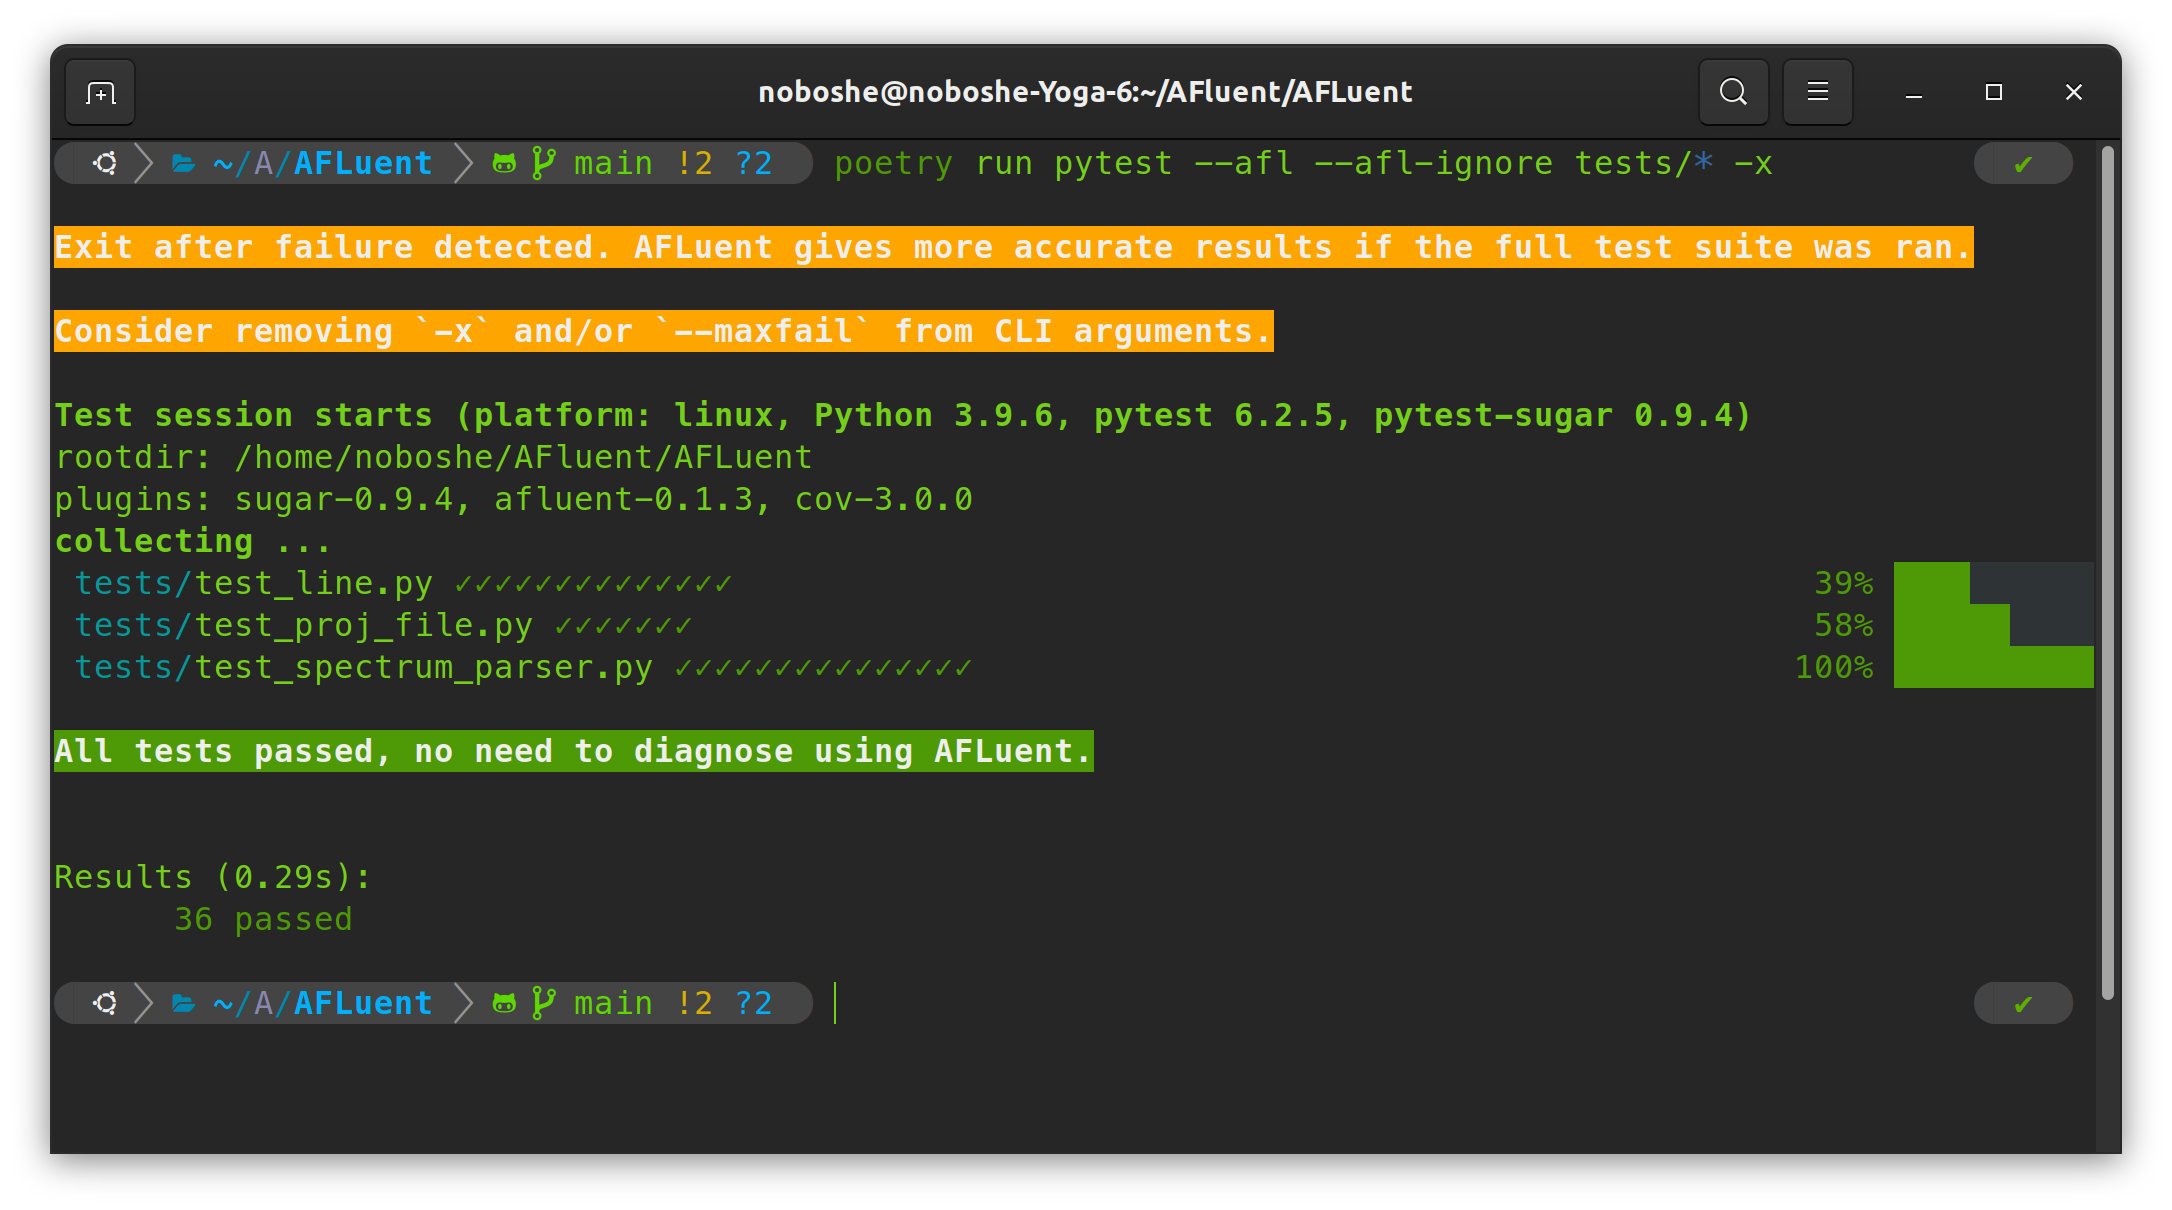
\includegraphics[width=15.5cm]{warning_message_1.png}
		\caption{\label{fig:warning_message_1} Maxfail Warning Message}
	\end{center}
\end{figure}

Another warning message is displayed when AFLuent is installed to the current
Python environment but not enabled by the user through the \code{---afl} or
\code{---afl-debug} flags. This message serves as a reminder to the user to
enable the plugin if they're interested in utilizing fault localization. The
message is shown in Fig\ref{fig:warning_message_2}.

\begin{figure}[!htb]
	\begin{center}
		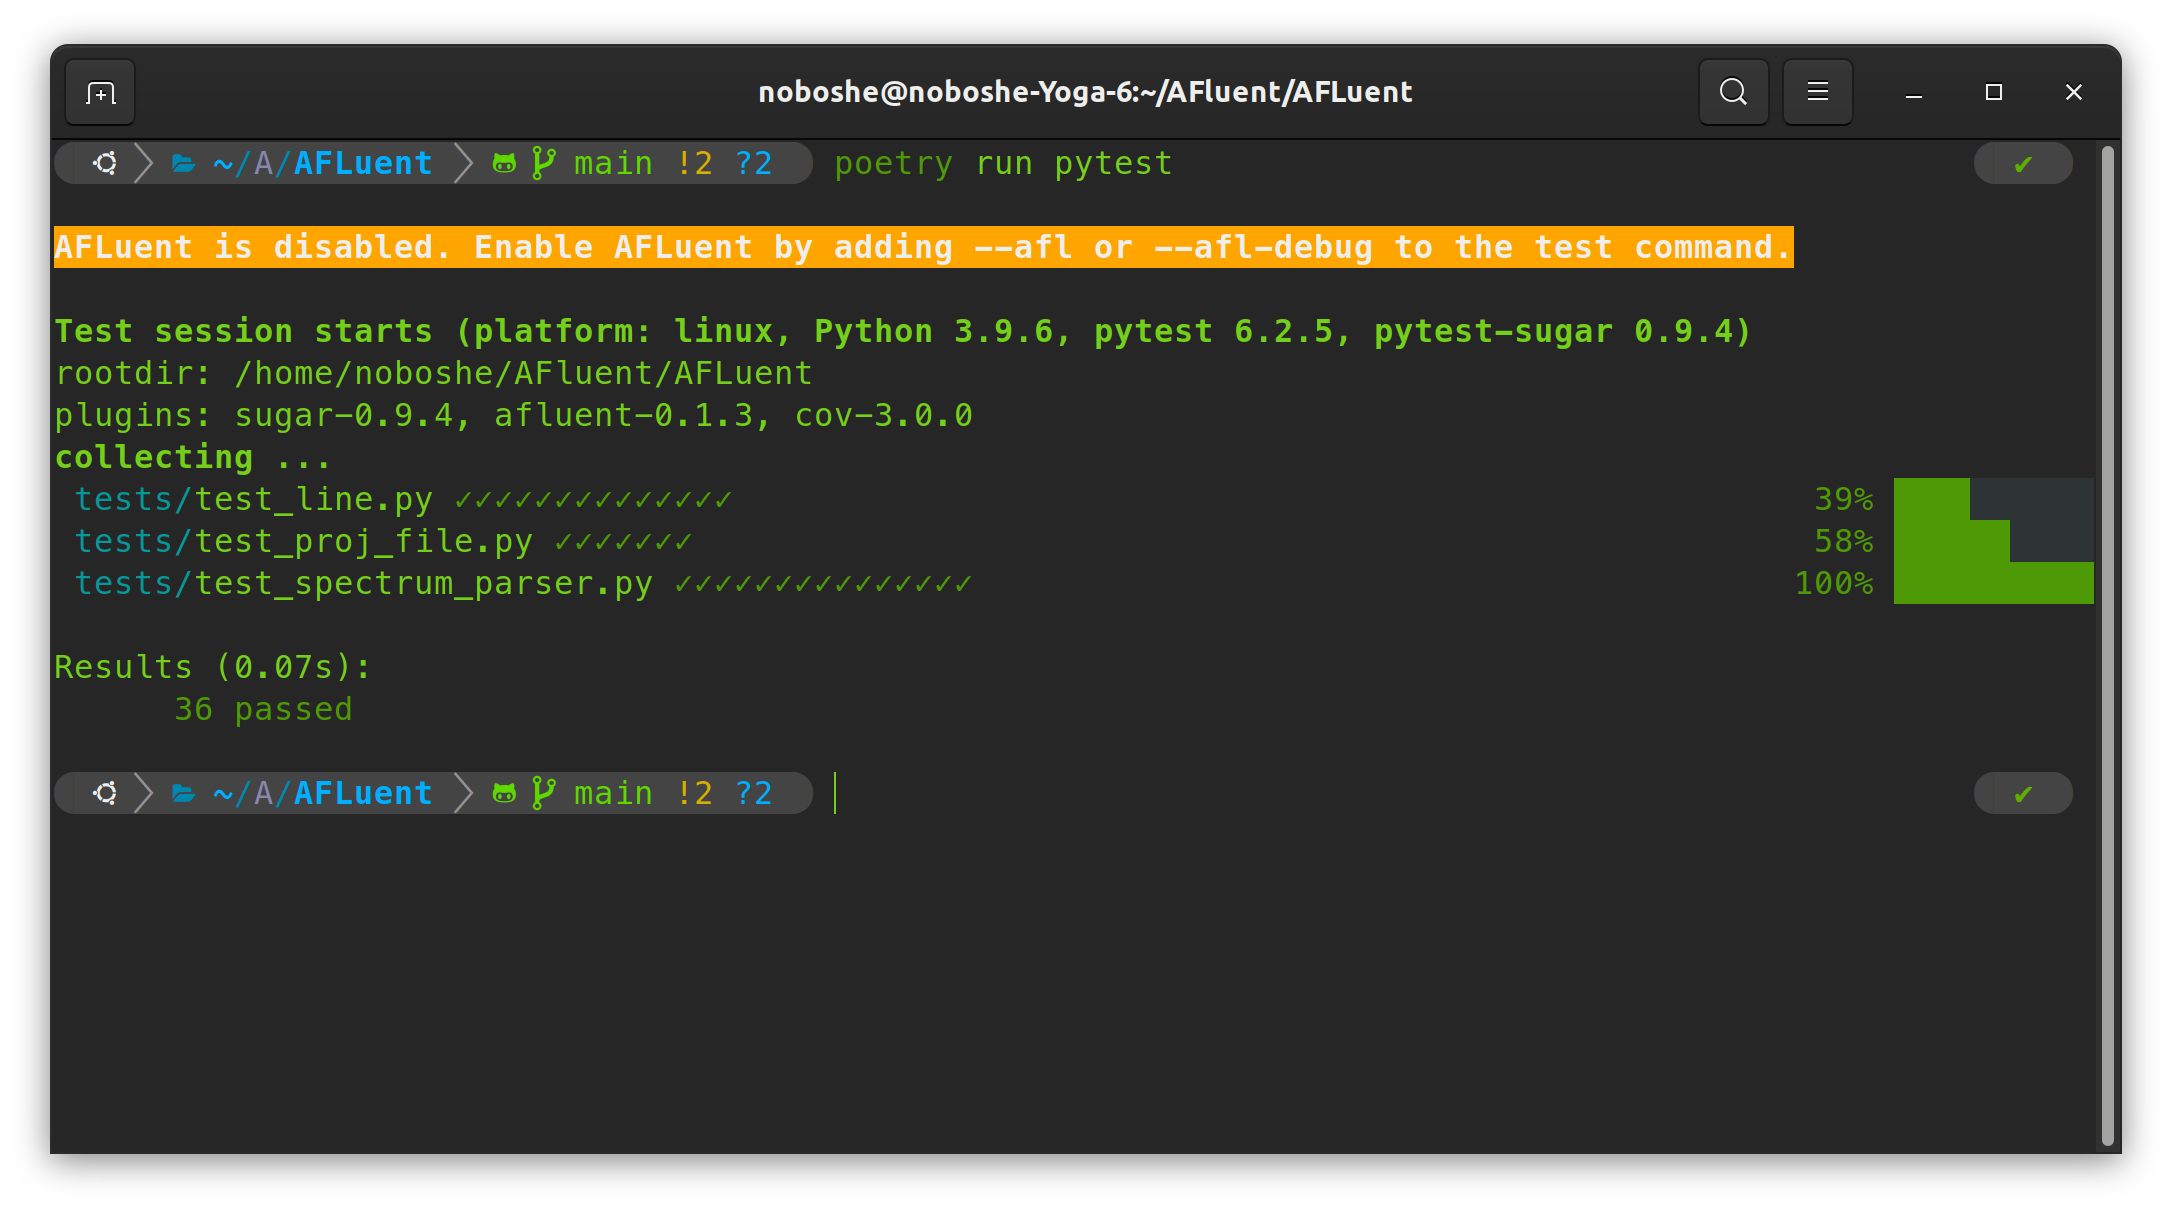
\includegraphics[width=15.5cm]{warning_message_2.png}
		\caption{\label{fig:warning_message_2} AFLuent Disabled Warning Message}
	\end{center}
\end{figure}

The third and last case that causes a warning message takes place when a potential
conflict with Coverage.py is detected. In the possibility that another coverage
collecting Pytest plugin is enabled in the same session as AFLuent, coverage
data could be mixed up leading to inaccurate results or internal errors in
Pytest. To avoid that, AFLuent scans the enabled plugins for the current session
and checks if \code{pytest-cov} is running. If so, a warning message is
displayed but the session continues as expected. It's recommended that when running
AFLuent, that \code{pytest-cov} is disabled from the command line. Moreover, when
running \code{pytest-cov}, it's safer to disable AFLuent. This can be done by
adding \code{-p no:pytest-cov} to disable \code{pytest-cov} or \code{-p
no:afluent} to disable AFLuent. There could potentially be many
other Pytest plugins that conflict with AFLuent, however, \code{pytest-cov} is
the only known one thus far.

\begin{figure}[!htb]
	\begin{center}
		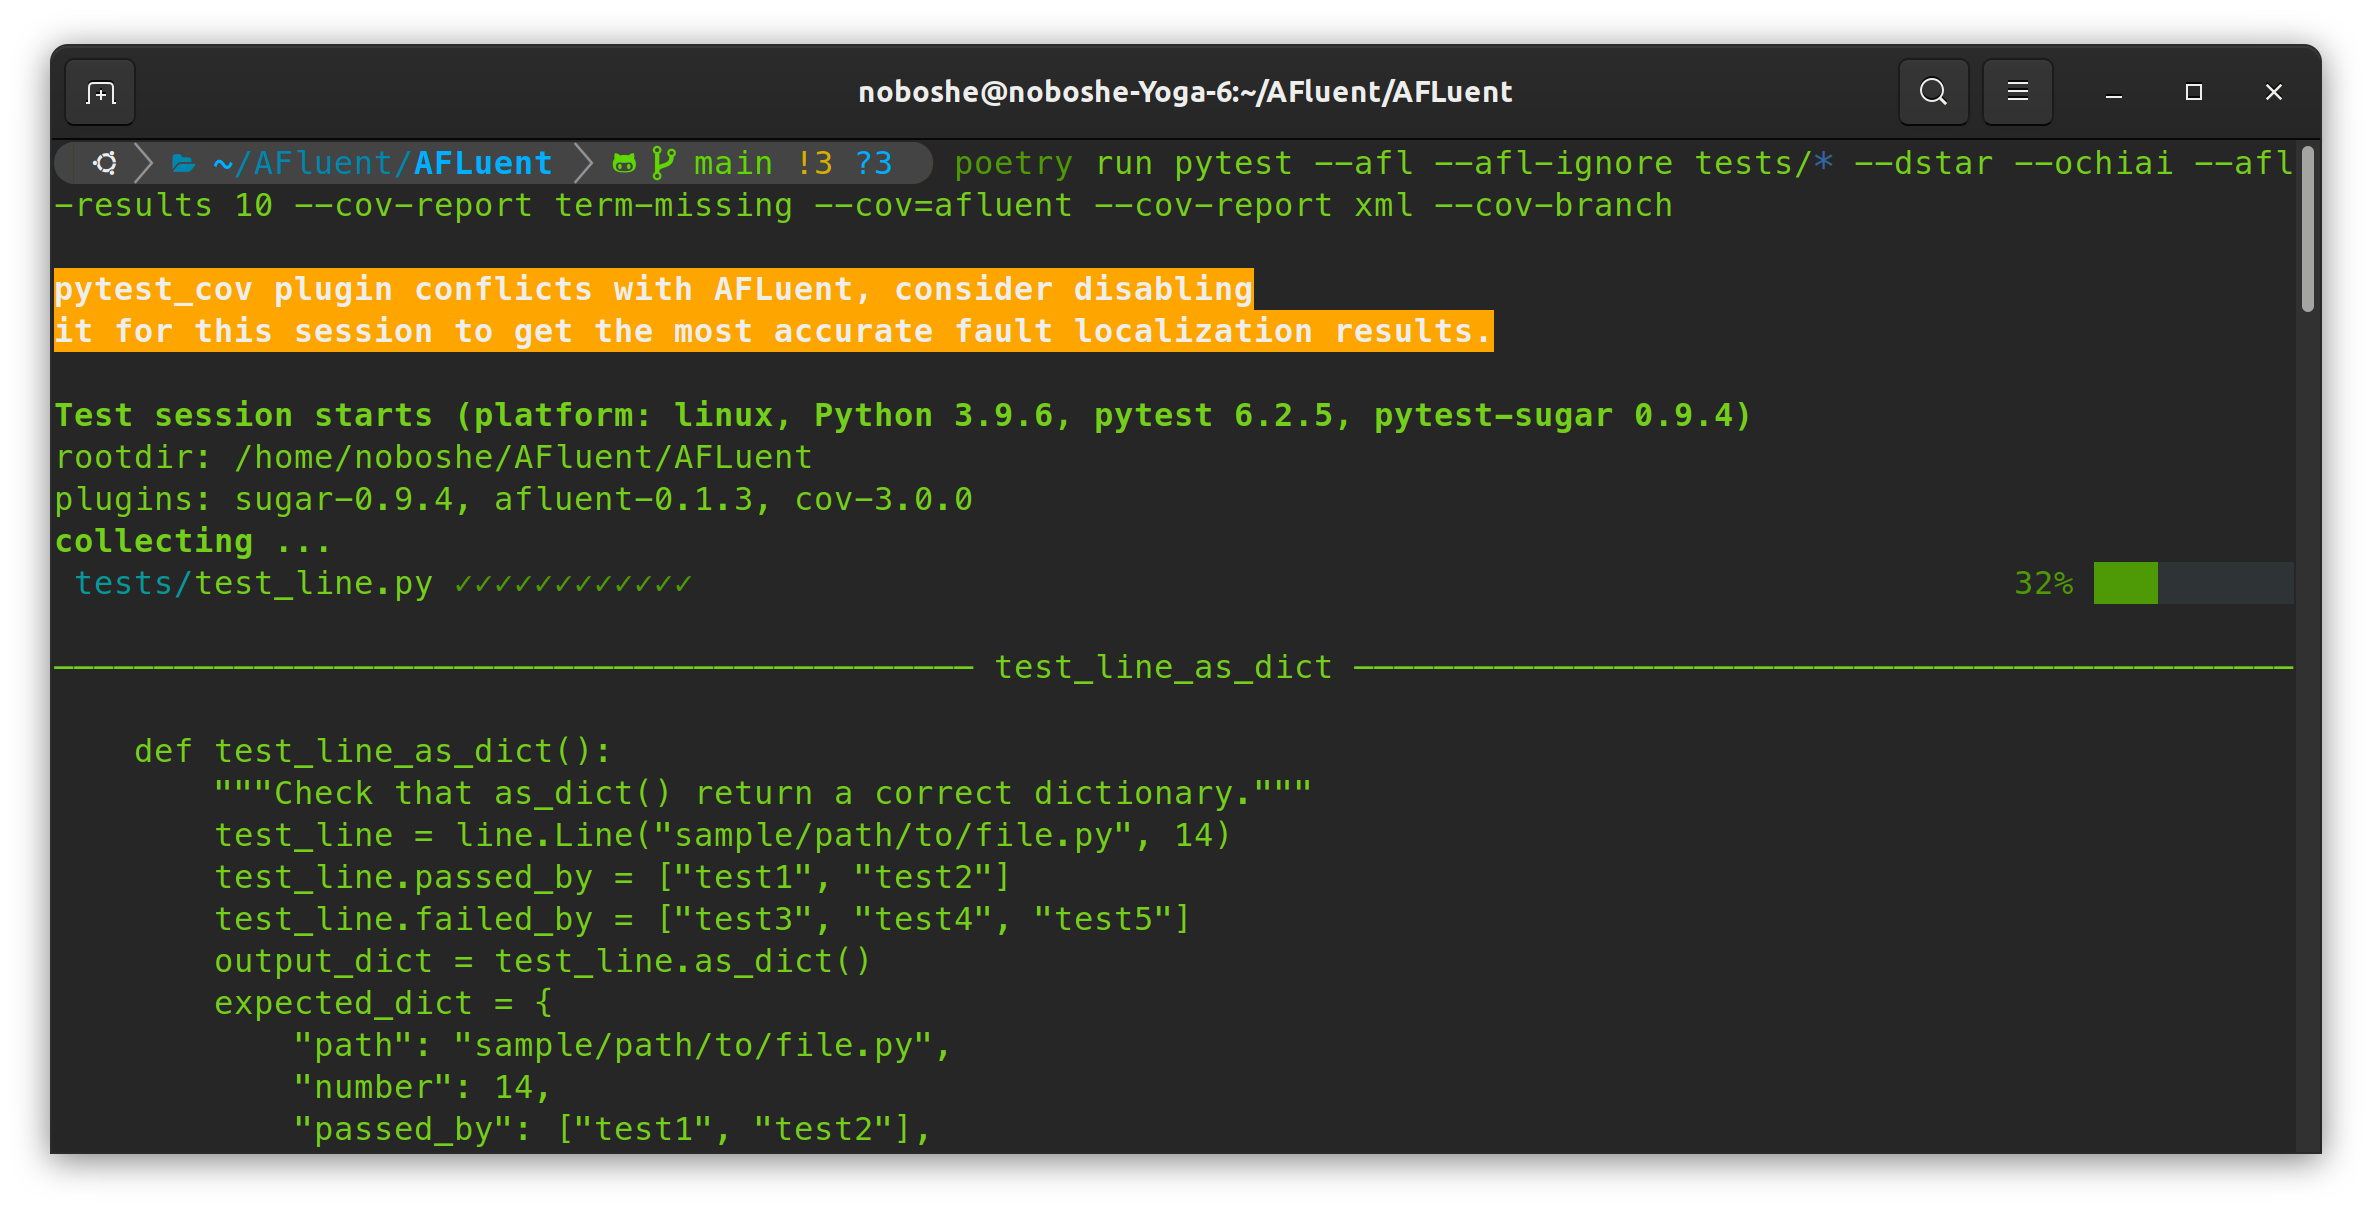
\includegraphics[width=15.5cm]{warning_message_3.png}
		\caption{\label{fig:warning_message_3} Conflicting Plugin Warning Message}
	\end{center}
\end{figure}

\subsection{Console Report}
\label{subsec:console_output}

In the case that AFLuent was enabled for the Pytest session and at least one
failure occurred, a report is generated and printed to the console to help the
user look for the error. Based on the inputs passed in the command-line
arguments, this report can be structured in many different ways. Generally, the
report is a table with rows containing the path to the file, the line number,
and suspiciousness score(s). The number of rows depends on the value of
\code{---afl-results} argument, which is set to 20 by default. Additionally, the
user can determine one or many equations to use for suspiciousness score
calculations, where the results will be sorted using the first one mentioned in
the command. For example, the command \code{poetry run pytest --afl --afl-ignore
tests/* --ochiai --dstar --afl-results 10} will display the top 10 results
sorted by the most suspicious using the Ochiai equation. However, the
DStar suspiciousness will also be displayed. Figure \ref{fig:report_1} shows an
example of the report when running the AFLuent test suite after introducing a
bug in the code.

\begin{figure}[!htb]
	\begin{center}
		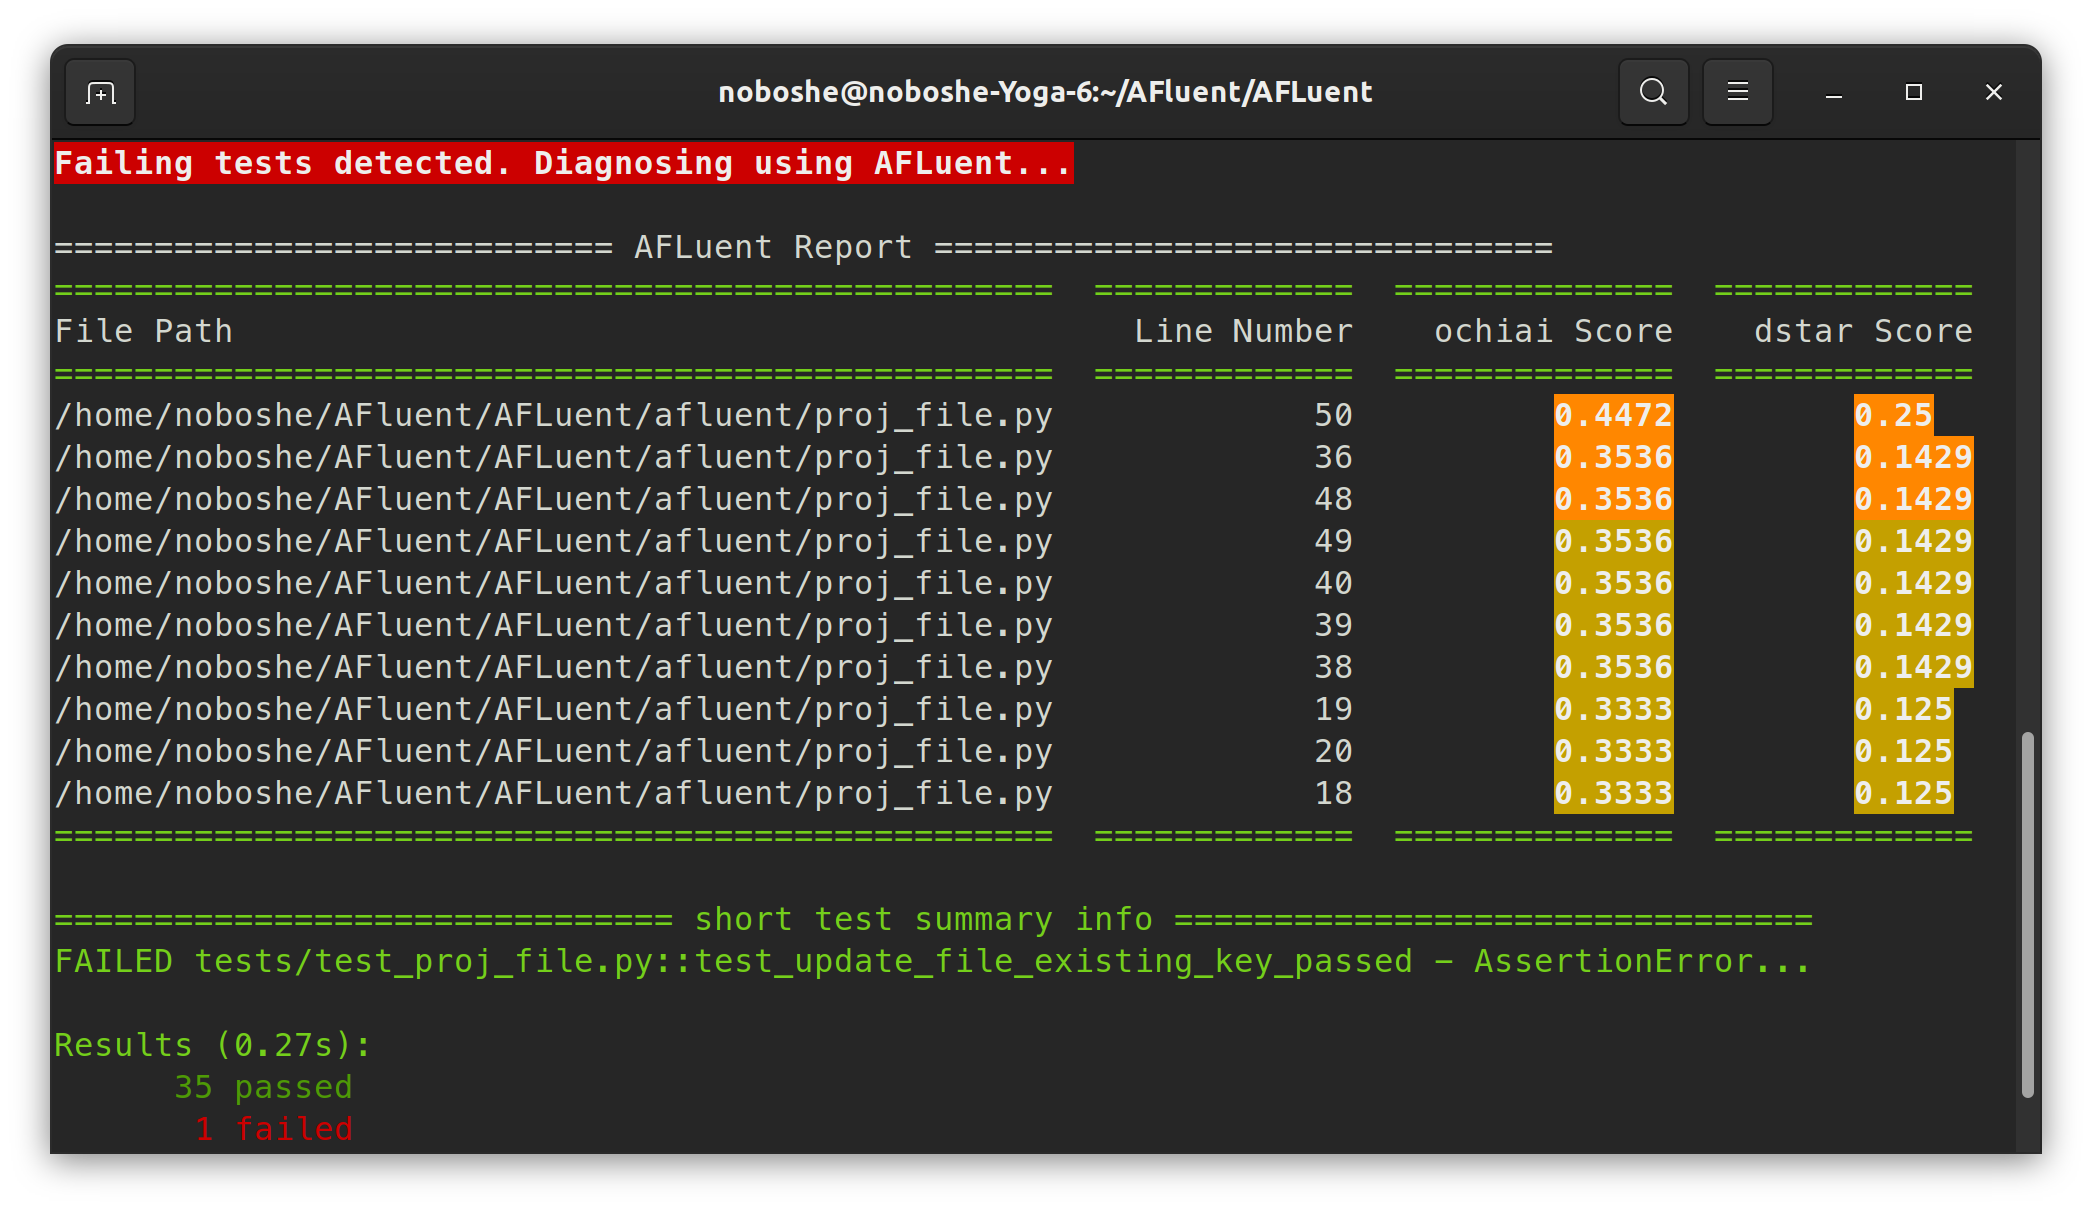
\includegraphics[width=15.5cm]{report_1.png}
		\caption{\label{fig:report_1} Example Report Using Ochiai and DStar}
	\end{center}
\end{figure}

In addition to printing the report, AFLuent color codes elements based on their
rankings. The four possible colors are green, yellow, orange, and red, where
each one represents the likelihood of finding the fault at that line.
Suspiciousness scores highlighted using green signify that the corresponding
element is safe and has a zero suspiciousness score. On the opposite end of the
spectrum, scores are highlighted with red when they equal the maximum
suspiciousness score possible (usually 1), the color indicates that these
elements are extremely likely to be the ones causing the fault. For the
remaining results, the top 20\% are highlighted using orange to show that they
are risky of being faulty. The remaining non-zero elements are highlighted using
yellow. Figure \ref{fig:report_2} shows an example of how safe statements are
displayed in the report.

\begin{figure}[!htb]
	\begin{center}
		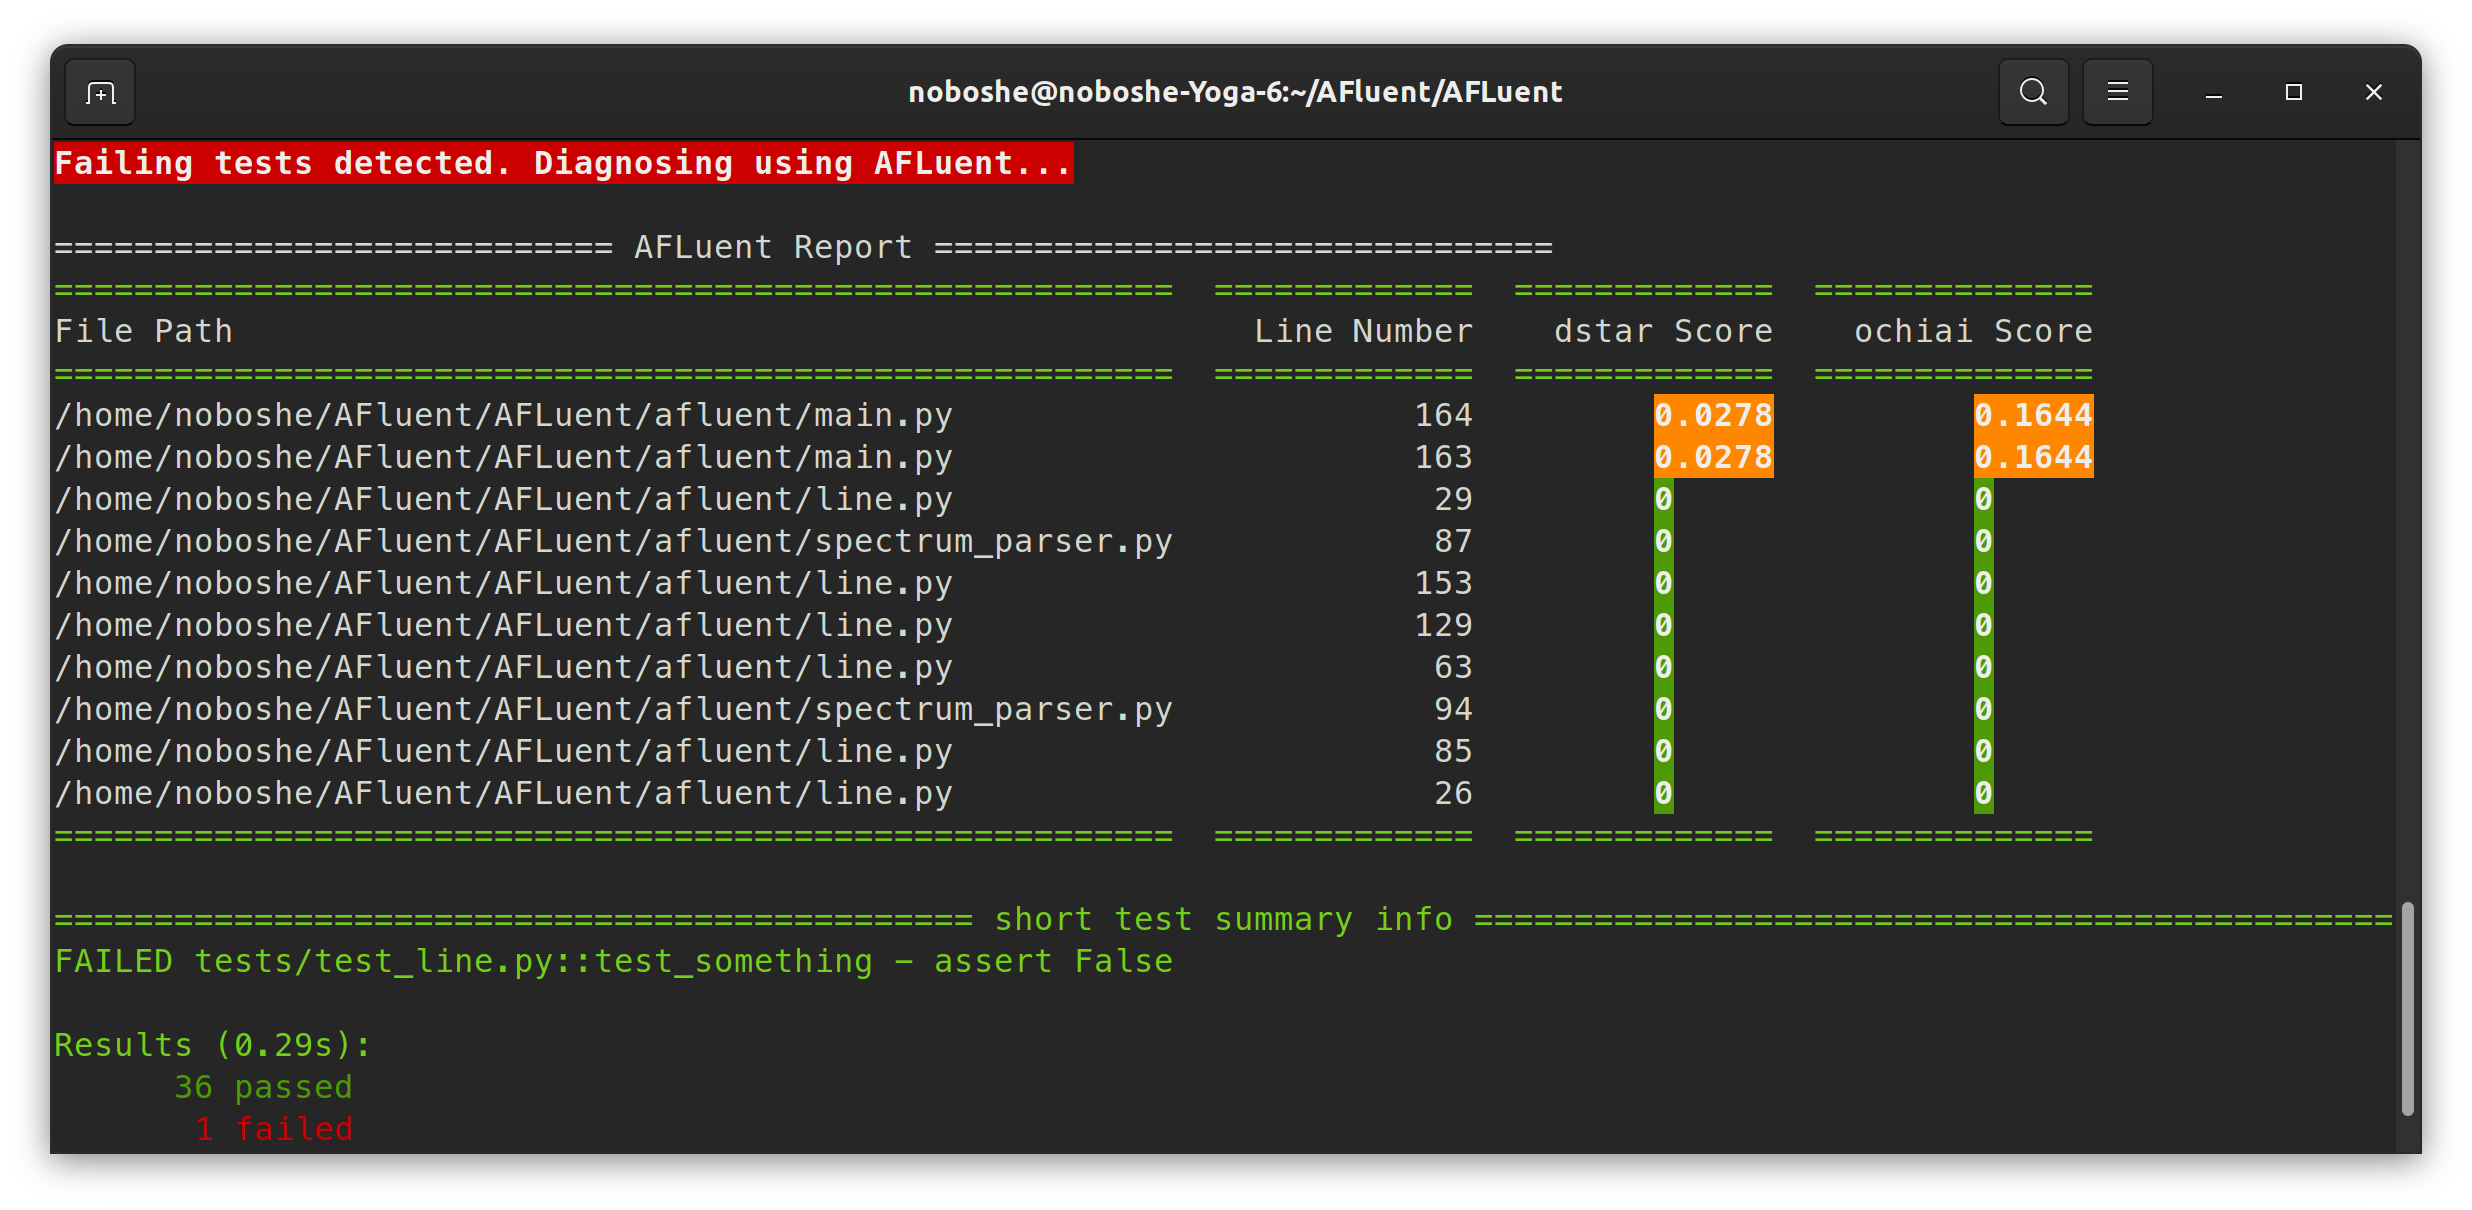
\includegraphics[width=15.5cm]{report_2.png}
		\caption{\label{fig:report_2} Example Report With Safe Statements}
	\end{center}
\end{figure}

\subsection{File Report}
\label{subsec:file_output}

Aside from the reports produced in the console, AFLuent can create report files
of the rankings in both JSON and CSV formats. Additional reporting of per-test
coverage is also possible. The command line arguments \code{–-report} and
\code{–-per-test-report} enable this feature. Producing these reports facilitates
the evaluation of AFLuent by allowing the storage of rankings in a file for
further analysis later on. In general, the standard report contains the rankings
of the lines using the approach requested by the user. Additionally, other
columns in the report contain the scores of all the other approaches for
comparison. On the other hand, the per-test report is a dictionary structured
such that the main keys are the names of the different test cases in the test
suite and the value is an object that stores the lines executed by that test
case as well as the outcome of the test.

\section{Tie Breaking}
\label{sec:tiebreaking}

Ties are a frequent issue in spectrum-based fault localization. They often cause
issues in identifying the source of the fault and render the scores useless. To
mitigate this problem, AFLuent implements three different approaches to resolve
the inevitable ties in suspiciousness scores. These techniques can hopefully
provide another metric to break the tie between two elements.

\subsection{Random}
\label{subsec:tiebreak_random}

Random tie breaking is the baseline approach for dealing with ties in
suspiciousness scores. It's the method to compare other approaches to in order
to detect if there are any improvements. In random tie breaking, statements are
ranked in a descending order by the chosen suspiciousness score first, however,
the order between tied elements is random. This could lead to different rankings
for each run of the tool.

\subsection{Cyclomatic Complexity}
\label{subsec:c_complexity}

One of the available ways to break ties between elements is to use cyclomatic
complexity as a secondary score to consider when sorting. This score is proposed
by McCabe \cite{cyclomatic_complexity} and can be easily calculated using the Radon library. It measures the number of available paths that execution
cold go through in a function. Since this type of score only applies to whole
functions and not to individual elements, lines inherit the cyclomatic
complexity score of the function they live in when being ranked.Essentially, if
a function has a cyclomatic complexity score of 7, then all statements within
the function also have that score. While this can help break many ties, it's not
effective in breaking ties when the tied elements exist in the same function.
However, further empirical evaluation of its performance will be discussed in
the evaluation section.

\subsection{Mutant Density: Logical Set}
\label{subsec:tiebreak_mutant_density_logical}

Another metric used to break ties between suspicious statements is mutant
density. More specifically, this score indicates how error prone the statement
is by calculating the number of all possible mutants. For example, a statement
that has many mathematical and logical operators to perform a calculation is
more error prone that a statement that only has one or two of these operations.
With that in mind, AFLuent uses this information to break ties between
statements that have the same suspiciousness score but are syntactically
different.

In the implementation of this approach, the focus was on mutants in logical
operations such as arithmetic, boolean, comparison operators, and others.
Table \ref{table:logical_set_mutants} includes all the possible mutants which
are considered with support from Libcst. The number of these operators is
calculated only for simple statements as defined by Libcst, therefore, it does
not include \code{if} statements, function definition, \code{while} loops and so on.

\begin{table}[!htb]
	\centering
	\begin{tabular}{|c|c|c|c|c|}
	 \hline
	 Unary & Boolean
	 & Binary  & Comparison & Augmented Assignment \\
	 \hline
	 BitInvert & And & Add & Equal & AddAssign\\
	 Not & Or & BitAnd & GreaterThan & BitAndAssign \\
	 Minus &  & BitOr & GreaterThanEqual & BitOrAssign \\
	 Plus &  & BitXor & In & BitXorAssign \\
	  &  & Divide & Is & DivideAssign \\
	  &  & FloorDivide & LessThan & FloorDivideAssign \\
	  &  & LeftShift & LessThanEqual & LeftShiftAssign \\
	  &  & MatrixMultiply & NotEqual & MatrixMultiplyAssign \\
	  &  & Modulo & IsNot & ModuloAssign \\
	  &  & Multiply & NotIn & MultiplyAssign \\
	  &  & Power &  & PowerAssign \\
	  &  & RightShift &  & RightShiftAssign \\
	  &  & Subtract &  & SubtractAssign \\
	 \hline
	\end{tabular}
	\caption{Mutants in the Logical Set}
	\label{table:logical_set_mutants}
\end{table}


\subsection{Mutant Density: Enhanced Set}
\label{subsec:tiebreak_mutant_density_enhanced}

This approach to tie breaking also uses mutant density evaluate how error prone
a statement is. However, it seeks to provide a more holistic metric that also
considers how error prone the constructs that an a statement is nested in. For
example, a statement inside a multi-level if statement, which is also nested in
a loop, is more error prone than a statement which is outside these constructs.
Since there is more room for errors in loops and if statement conditions, a
statement nested in them takes on this risk of error. In order to measure this
score, the list of mutant used in the logical set was extended to include
additional constructs that might contain the error. Additionally, the tiebreaker
looks through and scores each block that the statement is nested in.
Table\ref{table:enhanced_set_mutants} shows the additional mutants that are
looked for in the enhanced set. Additionally, Table\ref{table:construct_scoring}
discusses how a score is assigned to each construct while parsing through the
syntax tree and assessing how error prone a statement is. All of these
approaches are used to calculate a score that gets used in breaking ties of
suspicious statements while ranking. Figure\ref{fig:enhanced_score_equation}
shows how each construct score is used in generating the final score of a statement.

\begin{table}[!htb]
	\centering
	\begin{tabular}{|c|c|}
	 \hline
	 Mutant & Description \\
	 \hline
	 Annotated Assign & Assignment to a variable that contains type hints \\
	 Assign & Simple assignment to a variable using the single equal sign  \\
	 Function Call & A call to any function \\
	 Subscript & Indexing a list, dictionary, tuple or an object using brackets \\
	 Literal Tuple & Literal constructed tuple using parenthesis \\
	 Literal List & Literal constructed list using brackets \\
	 Literal String &  Literal constructed string using quotation marks \\
	 Literal Dictionary &  Literal constructed tuple using curly braces \\
	 Literal Integer &  Literal integer (not a variable that stores one) \\
	 Literal Float &  Literal float (not a variable that stores one) \\

	 \hline
	\end{tabular}
	\caption{Mutants in the Enhanced Set}
	\label{table:enhanced_set_mutants}
\end{table}

\begin{table}[!htb]
	\centering
	\begin{tabular}{|c|c|}
	 \hline
	 Construct & Scored Using \\
	 \hline
	 Function Definition & Number of arguments in the function signature \\
	 If statement & Number of enhanced list mutants in the test condition  \\
	 Simple statement & Number of the enhanced list mutants in the statement \\
	 While loop & Number of enhanced list mutants in the test condition \\
	 For loop & Number of enhanced list mutants in the iterator and iterable \\
	 With statement & Number of the enhanced list mutants in the statement \\

	 \hline
	\end{tabular}
	\caption{Construct Scoring in Enhanced Set}
	\label{table:construct_scoring}
\end{table}


\begin{figure}[!htb]
	\begin{center}
		\begin{equation}
			Score(statement) = \frac{\textbf{M$_{statement}$} + \frac{\textbf{M$_{c1}$ + M$_{c2}$ + ... + M$_{ci}$}}{\textbf{i}}}{2}
		\end{equation}
		\caption{\label{fig:enhanced_score_equation} Enhanced Score Equation}
	\end{center}
\end{figure}

\subsection{Tiebreaking Overview}
\label{subsec:tiebreak_overview}

\begin{table}[!htb]
	\begin{tabular}{|c|l|c|c|c|}
	 \hline
	 & Line
	 & Cyclomatic  & Logical & Enhanced \\
	 \hline
	 1: & \code{def some\_func(arg1, arg2, arg3, arg4: str):} & 3 & 0 & 2.0\\
	 2: & \qquad\code{int1 = arg1 * arg2 / arg3} & 3 & 2 & 3.5 \\
	 3: & \qquad\code{int2: str = arg4 + "hello world"} & 3 & 1 & 3.5 \\
	 4: & \qquad\code{my\_list = ["some item"]} & 3 & 0 & 3.5 \\
	 5: & \qquad\code{while int1 < 30:} & 3 & 0 & 1.5 \\
	 6: & \qquad\qquad\code{my\_list.append(int2)} & 3 & 0 & 2.0 \\
	 7: & \qquad\qquad\code{if len(my\_list) > 15:} & 3 & 0 & 1.5 \\
	 8: & \qquad\qquad\qquad\code{print("done")} & 3 & 0 & 2.5 \\
	 9: & \qquad\qquad\qquad\code{break} & 3 & 0 & 1.5 \\
	 10: & \qquad\code{with open("my\_file.txt", "w+") as outfile:} & 3 & 0 & 1.0 \\
	 11: & \qquad\qquad\code{outfile.write(str(my\_list))} & 3 & 0 & 2.0 \\
	 12: &  & 0 & 0 & 0 \\
	 13: &  & 0 & 0 & 0 \\
	 14: & \code{def some\_other\_func(arg1, arg2):} & 4 & 0 & 1 \\
	 15: & \qquad\code{if arg1 > arg2:} & 4 & 0 & 0.75 \\
	 16: & \qquad\qquad\code{if 2 * arg2 > arg1:} & 4 & 0 & 1 \\
	 17: & \qquad\qquad\qquad\code{print(arg1)} & 4 & 0 & 1.5 \\
	 18: & \qquad\qquad\code{elif 3 * arg2 > arg1:} & 4 & 0 & 1.125 \\
	 19: & \qquad\qquad\qquad\code{print(arg2)} & 4 & 0 & 1.625 \\
	 20: & \qquad\code{else:} & 4 & 0 & 0.75 \\
	 21: & \qquad\qquad\code{print(arg1 * 3.5)} & 4 & 1 & 2.25 \\
	 \hline
	\end{tabular}
	\caption{Tiebreaking Score Examples}
	\label{table:scoring_examples}
\end{table}

Using all the tie breaking approaches discussed previously, this subsection
provides an overview and an example that demonstrates tie breaking on a sample
program. Table\ref{table:scoring_examples} shows a sample program that implement
two functions with some conditional logic and simple mathematical operations. It also
contains three columns with each scoring approach. Starting with the cyclomatic
scores, one can see that all statements in a function contain the same score.
This number represents the cyclomatic complexity of the function resulting from
using Radon. While this approach is expected to break ties, it could potentially
fail at doing so if the tied statements are in the same function. As for the
logical approach scoring, it only applies to simple statements such as lines
2,3,4,6,8,11,17,19, and 21. Using this approach, mutant density is calculated
using logical mutants only. For example, since line 2 contains the two binary
operators \code{*} and \code{/} for multiplication and division, the mutant
density of the statement is 2, which is also its   score. Note that
variable assignment and literals do not affect logical tie breaking scores.
Lastly, enhanced tie breaking takes into consideration a more extensive list of
possible mutants. Additionally, it analyzes a wider range of statements that
include if statements, while and for loops, as well as function definitions.
Using some examples from the sample program in
Table\ref{table:scoring_examples}, the enhanced score for line 3 would be
calculated as follows:
$$\frac{\textbf{3 + (4 / 1)}}{2}$$
Where 3 is the number
of enhanced list mutants in the line (annotated assign, plus, literal string), 4
is the total number of enhanced list mutants the statement is nested in, and 1
is the total number of constructs that the statement is nested in. Using another
example on line 8, the score would be calculated as follows:
$$\frac{\textbf{2 + (9 / 3)}}{2}$$
Where 2 is the number of possible mutants in the statement itself (function
call, and literal string), 9 is the total number of possible mutants in
constructs that the statement is nested in (len() , >, 15, <, 30, four function
arguments) and 3 is the number of constructs that the statement is nested in (if
statement, while loop, and function). Using the same process the enhanced score
is calculated for all the lines in the program and used for breaking ties in
suspiciousness scores.
